% !TEX root = Projektdokumentation.tex
\section{Anhang}


\subsection{Berechnung des Stundensatzes von Mitarbeitenden}
\label{app:Stundensatz}
Nach der Entgeldtabelle der IG Metall Bayern für Metall und Elektro\footnote{Vgl. \cite{Entgeldtabelle}} erhalten Angestellte der Entgeldgruppe EG 08 ein Monatsbruttogehalt von \eur{3.800,00}. Zusätzlich dazu müssen ungefähr ein Fünftel für die Arbeitgeberanteile der Sozialversicherung und Mehrleistungen wie Urlaubsgeld hinzugerechnet werden.\footnote{Vgl. \cite{Personalkosten}} Aufsummiert ergibt das jährliche Personalkosten von \eur{54.720,00}.

\begin{eqnarray}
\eur{3.800,00} \cdot 1,2 \cdot 12 \mbox{ m} = \eur{54.720,00} \mbox{ /a}
\end{eqnarray}

Eine Arbeitszeit von 35 Stunden pro Woche bedeuetet bei 52 Wochen eine Jahresarbeitszeit von 1820 Stunden. Abzüglich der Urlaubstage (30), Feiertage (ca. 11) und Fehltage durch Krankheit und Fortbildungen (ca. 15) ergibt das eine Jahresarbeitszeit von 1498 Stunden pro Jahr.

\begin{eqnarray}
35 \mbox{h/w} \cdot 52 \mbox{ m} = 1820 \mbox{ h/a} \\
1820 \mbox{ h/a} - [(30+11+15) \mbox{d} \cdot 35 \mbox{h/d}] = 1498 \mbox{ h/a}
\end{eqnarray}

Werden die Jahrespersonalkosten von \eur{54.720,00} durch die Jahresarbeitszeit von 1498 Stunden dividiert, ergibt dies Stundenkosten für den Arbeitgeber in Höhe von \eur{36,53}. Da es sich hierbei um eine Schätzung handelt, wird vereinfacht von \eur{40,00} pro Stunde ausgegangen.  

\begin{eqnarray}
\eur{54.720,00} /a \div 220 \mbox{ h/a} = \eur{36,53} /h \approx \eur{40,00} /h 
\end{eqnarray}

Für Auszubildende mit einer Ausbildungsvergütung in Höhe von \eur{1.207,00} \footnote{Vgl. \cite{EntgeldtabelleAzubis}} ergeben sich nach selber Kalkulation Personalkosten in Höhe von \eur{10,57}, also vereinfacht \eur{10,00} pro Stunde.

\begin{eqnarray}
25 \cdot 220 \mbox{ Tage/Jahr} \cdot 10 \mbox{ min/Tag} = 55000 \mbox{ min/Jahr} \approx 917 \mbox{ h/Jahr} 
\end{eqnarray}
\clearpage

\subsection{Installationsskript für Ubuntu 18.04}
\label{app:skript}

\# Systemupdate \\
apt update\\
apt dist-upgrade\\

\# Grundinstallation icinga und MySQL\\
apt install icinga2 icingacli monitoring-plugins mysql-server mysql-client\\
mysql\_{}secure\_{}installation\\

\# Installation Icinga IDO und Web-Interface\\
apt install icinga2-ido-mysql\\
apt install icingaweb2\\

\# Klonen Github-Repository\\
cd /usr/share\\
mv icingaweb2 old.icingaweb2\\
git config --global http.proxy http://webproxy1.kuka.int.kuka.com:80\\
git clone https://github.com/Icinga/icingaweb2.git\\

\# Installation fehlendes PHP-Plugin\\
apt install php7.2-curl\\
systemctl restart apache2\\

\# Hinzufügen MySQL User für icingaweb2\\
mysql -e "CREATE USER 'icingaweb'@'localhost' IDENTIFIED BY '•••';"\\
mysql -e "GRANT ALL PRIVILEGES ON *.* TO 'icingaweb'@'localhost';"\\
mysql -e "FLUSH PRIVILEGES;"\\

\# Einrichtungstoken erstellen\\
icinga2 feature enable command ido-mysql\\
icingacli setup token create\\
systemctl restart icinga2\\
\clearpage

\subsection{Screenshots}
\label{Screenshots}

\begin{figure}[htb]
\centering
\includegraphicsKeepAspectRatio{screen_vmnetwork.jpg}{0.9}
\caption{Netzwerkkonfiguration in VMware ESXi. (Rechts physische Netzwerkport, links virtuelle Ports der VMs, mitte ein virtueller Switch)}
\label{screen:vmnetwork}
\end{figure}

\begin{figure}[htb]
\centering
\includegraphicsKeepAspectRatio{screen_vmcreation.jpg}{0.9}
\caption{Parameteranpassung bei Erstellung einer virtuellen Maschine in VMware ESXi}
\label{screen:vmcreation}
\end{figure}
\clearpage

\begin{figure}[!htb]
\centering
\includegraphicsKeepAspectRatio{screen_mysqlsecure.jpg}{0.9}
\caption{Das Skript \glqq{}mysql\_{}secure\_{}installation\grqq{} zur Absicherung eines MySQL-Systems}
\label{screen:mysqlsecure}
\end{figure}

\begin{figure}[!htb]
\centering
\includegraphicsKeepAspectRatio{screen_phperror.jpg}{1}
\caption{PHP-Fehler nach Installation des Icinga-Webfrontends}
\label{screen:phperror}
\end{figure}

\begin{figure}[!htb]
\centering
\includegraphicsKeepAspectRatio{screen_konfigassistent.jpg}{1}
\caption{Willkommens-Bildschirm des Konfigurationsassistenten}
\label{screen:konfigassistent}
\end{figure}

\begin{figure}[!htb]
\centering
\includegraphicsKeepAspectRatio{screen_userdb.jpg}{1}
\caption{Einrichtung der Datenbank für Webfrontend-Benutzer}
\label{screen:userdb}
\end{figure}

\begin{figure}[!htb]
\centering
\includegraphicsKeepAspectRatio{screen_landingpage.jpg}{1}
\caption{Startseite von \glqq{}Icinga 2\grqq{} nach der Erstkonfiguration. Der Server, auf dem die Instanz von \glqq{}Icinga 2\grqq{} läuft, ist automatisch als erster Server hinzugefügt}
\label{screen:landingpage}
\end{figure}

\begin{figure}[!htb]
\centering
\includegraphicsKeepAspectRatio{screen_newservers.jpg}{1}
\caption{Konfiguration in \code{/etc/icinga2/conf.d/hosts.conf} um zwei neue Server dem Monitoring hinzuzufügen}
\label{screen:newservers}
\end{figure}

\begin{figure}[!htb]
\centering
\includegraphicsKeepAspectRatio{screen_loaddefinition.jpg}{0.5}
\caption{Beispiel für ein definiertes \glqq{}CheckCommand\grqq{}-Objekt}
\label{screen:loaddefinition}
\end{figure}

\begin{figure}[!htb]
\centering
\includegraphicsKeepAspectRatio{screen_service.png}{0.5}
\caption{Beispiel für einen definierten Dienst}
\label{screen:service}
\end{figure}

\begin{figure}[!htb]
\centering
\includegraphicsKeepAspectRatio{screen_webserver.png}{0.5}
\caption{Detailansicht eines überprüften Dienstes; hier die Webserverüberwachung}
\label{screen:webserver}
\end{figure}

\begin{figure}[!htb]
\centering
\includegraphicsKeepAspectRatio{screen_dashboard.png}{0.9}
\caption{Selbsterstelltes Dashboard}
\label{screen:dashboard}
\end{figure}



\subsection{Detaillierte Zeitplanung}
\label{app:Zeitplanung}

\tabelleAnhang{ZeitplanungKomplett}


\clearpage

\subsection{Use Case-Diagramm}
\label{app:UseCase}
Use Case-Diagramme und weitere \acs{UML}-Diagramme kann man auch direkt mit \LaTeX{} zeichnen, siehe \zB \url{http://metauml.sourceforge.net/old/usecase-diagram.html}.
\begin{figure}[htb]
\centering
\includegraphicsKeepAspectRatio{UseCase.pdf}{0.7}
\caption{Use Case-Diagramm}
\end{figure}



\subsection{Datenbankmodell}
\label{app:Datenbankmodell}
ER-Modelle kann man auch direkt mit \LaTeX{} zeichnen, siehe \zB \url{http://www.texample.net/tikz/examples/entity-relationship-diagram/}.
\begin{figure}[htb]
\centering
\includegraphicsKeepAspectRatio{database.pdf}{1}
\caption{Datenbankmodell}
\end{figure}
\clearpage

\subsection{Oberflächenentwürfe}
\label{app:Entwuerfe}
\begin{figure}[htb]
\centering
\includegraphicsKeepAspectRatio{MockupModules.pdf}{0.7}
\caption{Liste der Module mit Filtermöglichkeiten}
\end{figure}

\begin{figure}[htb]
\centering
\includegraphicsKeepAspectRatio{MockupModul.pdf}{0.7}
\caption{Anzeige der Übersichtsseite einzelner Module}
\end{figure}

\begin{figure}[htb]
\centering
\includegraphicsKeepAspectRatio{MockupTag.pdf}{0.7}
\caption{Anzeige und Filterung der Module nach Tags}
\end{figure}

\clearpage
\subsection{Entwicklerdokumentation}
\label{app:Doc}
\begin{center}
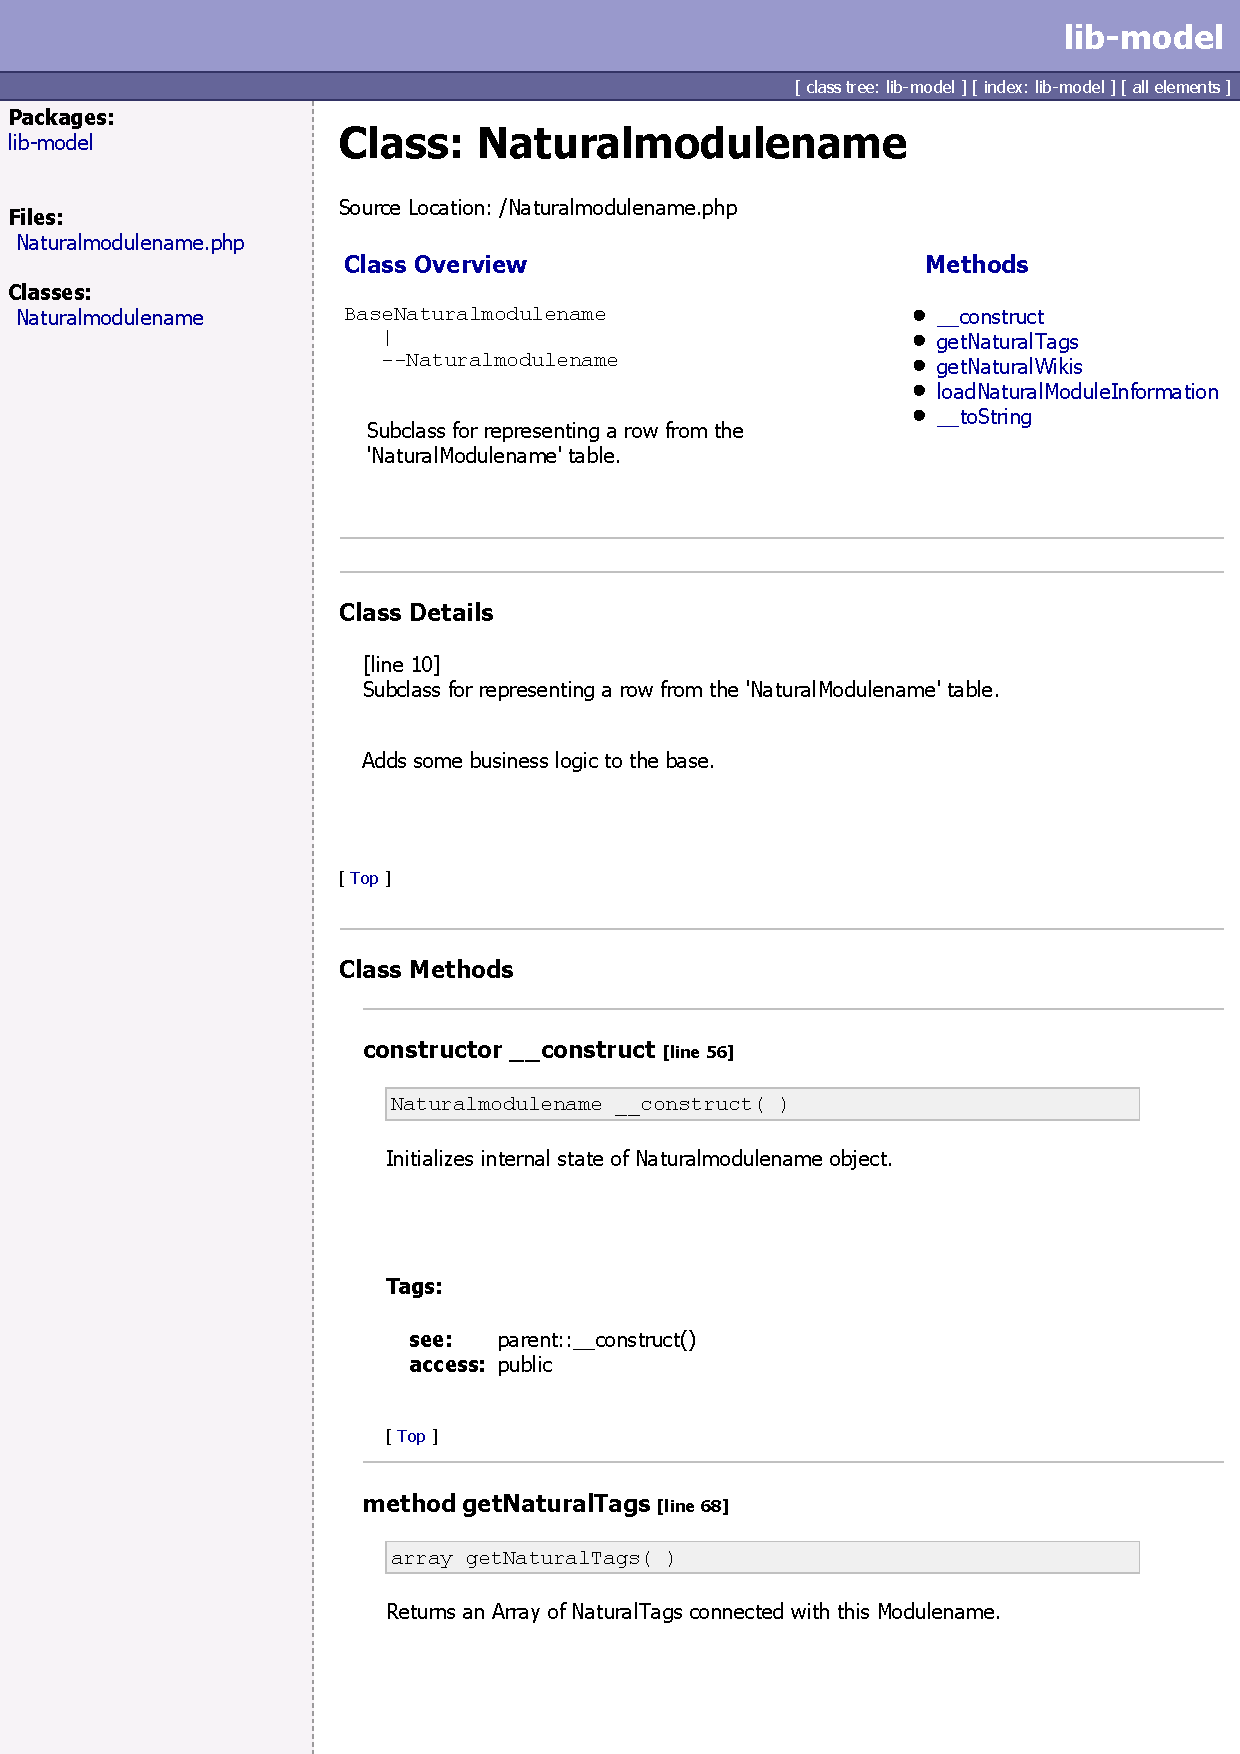
\includegraphics[page=1, width=0.9\textwidth]{doc.pdf}

\includegraphics[page=2, width=0.9\textwidth]{doc.pdf}
\end{center}

\clearpage
\subsection{Testfall und sein Aufruf auf der Konsole}
\label{app:Test}
\lstinputlisting[language=php, caption={Testfall in PHP}]{Listings/tests.php}
\clearpage
\begin{figure}[htb]
\centering
\includegraphicsKeepAspectRatio{testcase.jpg}{1}
\caption{Aufruf des Testfalls auf der Konsole}
\end{figure}


\subsection{Klasse: ComparedNaturalModuleInformation}
\label{app:CNMI}
Kommentare und simple Getter/Setter werden nicht angezeigt.
\lstinputlisting[language=php, caption={Klasse: ComparedNaturalModuleInformation}]{Listings/cnmi.php}
\clearpage

\subsection{Klassendiagramm}
\label{app:Klassendiagramm}
Klassendiagramme und weitere \acs{UML}-Diagramme kann man auch direkt mit \LaTeX{} zeichnen, siehe \zB \url{http://metauml.sourceforge.net/old/class-diagram.html}.
\begin{figure}[htb]
\centering
\includegraphicsKeepAspectRatio{Klassendiagramm.pdf}{1}
\caption{Klassendiagramm}
\end{figure}
\clearpage

\subsection{Benutzerdokumentation}
\label{app:BenutzerDoku}
Ausschnitt aus der Benutzerdokumentation:

\begin{table}[htb]
\begin{tabularx}{\textwidth}{cXX}
\rowcolor{heading}\textbf{Symbol} & \textbf{Bedeutung global} & \textbf{Bedeutung einzeln} \\
\includegraphicstotab[]{weather-clear.png} & Alle Module weisen den gleichen Stand auf. & Das Modul ist auf dem gleichen Stand wie das Modul auf der vorherigen Umgebung. \\
\rowcolor{odd}\includegraphicstotab[]{weather-clear-night.png} & Es existieren keine Module (fachlich nicht möglich). & Weder auf der aktuellen noch auf der vorherigen Umgebung sind Module angelegt. Es kann also auch nichts übertragen werden. \\
\includegraphicstotab[]{weather-few-clouds-night.png} & Ein Modul muss durch das Übertragen von der vorherigen Umgebung erstellt werden. & Das Modul der vorherigen Umgebung kann übertragen werden, auf dieser Umgebung ist noch kein Modul vorhanden. \\
\rowcolor{odd}\includegraphicstotab[]{weather-few-clouds.png} & Auf einer vorherigen Umgebung gibt es ein Modul, welches übertragen werden kann, um das nächste zu aktualisieren. & Das Modul der vorherigen Umgebung kann übertragen werden um dieses zu aktualisieren. \\
\includegraphicstotab[]{weather-storm.png} & Ein Modul auf einer Umgebung wurde entgegen des Entwicklungsprozesses gespeichert. & Das aktuelle Modul ist neuer als das Modul auf der vorherigen Umgebung oder die vorherige Umgebung wurde übersprungen. \\
\end{tabularx}
\end{table}


